\documentclass[authordate, empirical, issue]{jote-new-article}

\usepackage{caption}

\usepackage{tabularx}

\usepackage{graphicx}

\usepackage{hyperref}

\usepackage[backend=biber,style=apa]{biblatex}

\addbibresource{bibliography.bib}

\jotetitle{“But I didn’t understand your handwriting”! Uncovering the Significance of Therapy Progress Notes for Parents in Music Therapy}
\keywordsabstract{music therapy, progress notes, early intervention, power imbalances, parent}
\abstracttext{In this piece, I will explore a mistake I made by randomly handing a progress note to a parent at the end of a music therapy session, while overlooking the power imbalances embedded in such an act. I will share a clinical vignette involving Xavier\footnotemark, the father of a little girl named Blossom, who was only 10 months old, had many physical challenges, had severely impaired eyesight, and at the time could only sparsely respond to her loving environment. I will begin by describing a moment in the session when the father expressed his frustration from not being able to understand my handwriting in the progress note handed to him. Then, I will explore the unattended, underlying cultural and relational gaps in therapy that were captured in the virtually unnoticed gesture of handing a parent a scribbled progress note. Finally, I will examine the therapeutic requests expressed in such an important critique, which I failed to acknowledge as the family's therapist, focusing on aspects relating specifically to music therapy.}
\runningauthor{Hadar}
\jname{Journal of Trial \& Error}
\jyear{2023}
\paperreceived{May 13, 2023}
\paperaccepted{October 9, 2023}
\paperpublished{December 22, 2023}
\paperpublisheddate{2023-12-22}
\paperissued{December 22, 2023}
\paperdoi{10.36850/epwz-jj23}
\author[1]{\mbox{Tamar Hadar\orcid{0000-0003-1765-0360}}}
\affil[1]{Western Galilee College; University of Haifa}
\corremail{\href{mailto:tamarh@wgalil.ac.il}{tamarh@wgalil.ac.il}}
\corraddress{Western Galilee College; University of Haifa}
\runningauthor{Hadar}
\jwebsite{https://journal.trialanderror.org}

\articletype{Untangling Strings - Clinical Vignette}
\specialissue{Untangling Strings -- Further Explorations of Mistakes in Music Therapy}

\jvolume{3}
\jissue{2}
\jpages{44--48}

\begin{filecontents}{bibliography.bib}
	@article{Chifa2021,
    title       = {The soundscape of neonatal intensive care: {A} mixed-methods study of the parents},
    author      = {Chifa, M. and Hadar, T. and Politimou, N. and Reynolds, G. and Franco, F.},
    number      = {8},
    volume      = {8},
    url         = {https://doi.org/10.3390/children8080644.},
    doi         = {10.3390/children8080644.},
    date        = {2021},
    pages       = {644}
}


@article{Epstein2022,
    title       = {Israeli parents' lived experiences of music therapy with their preterm infants post-hospitalization},
    author      = {Epstein, S. and Elefant, C. and Ghetti, C.},
    number      = {3},
    volume      = {59},
    url         = {https://doi.org/10.1093/jmt/thac006},
    doi         = {10.1093/jmt/thac006},
    date        = {2022},
    pages       = {239--268},
    journal     = {The Journal of Music Therapy}
}


@article{Hadar2022,
    title       = {What sound does a cat make in Cantonese?”: {A}dvocating for lingual plurality in music therapy settings. Voices: {A} World Forum for Music Therapy, 22(3},
    author      = {Hadar, T.},
    url         = {https://doi.org/10.15845/voices.v22i3.3483},
    doi         = {10.15845/voices.v22i3.3483},
    date        = {2022}
}


@book{Hadar2023,
    title       = {Singing or playing the flute? Parents' perceptions of two different settings for parent-infant music groups},
    author      = {Hadar, T. and Politimou, N. and Franco, F.},
    url         = {https://doi.org/10.1177/03057356231166759},
    doi         = {10.1177/03057356231166759},
    publisher   = {Psychology of Music},
    date        = {2023}
}


@article{Inhestern2020,
    title       = {Parents' perception of their children's process of reintegration after childhood cancer treatment},
    author      = {Inhestern, L. and Peikert, M. L. and Krauth, K. A. and Escherich, G. and Rutkowski, S. and Kandels, D. and Bergelt, C.},
    number      = {10},
    volume      = {15},
    url         = {https://doi.org/10.1371/journal.pone.0239967},
    doi         = {10.1371/journal.pone.0239967},
    date        = {2020},
    pages       = {0239967-- 0239967},
    journal     = {PloS One}
}


@article{Kobus2021,
    title       = {Parents' perception of family-centered music therapy with stable preterm infants},
    author      = {Kobus, S. and Diezel, M. and Huening, B. and Dewan, M. V. and Felderhoff-Mueser, U. and Bruns, N.},
    number      = {23},
    volume      = {18},
    url         = {https://doi.org/10.3390/ijerph182312813},
    doi         = {10.3390/ijerph182312813},
    date        = {2021},
    pages       = {12813},
    journal     = {International Journal of Environmental Research and Public Health}
}


@article{Lindblad2016,
    title       = {Verbal dialogue in music therapy: {A} hermeneutical analysis of three music therapy sessions. Voices: {A} World Forum for Music Therapy, 16(1},
    author      = {Lindblad, K.},
    url         = {https://doi.org/10.15845/voices.v16i1.842},
    doi         = {10.15845/voices.v16i1.842},
    date        = {2016}
}


@inbook{Perilli2017,
    author      = {Perilli, G. G.},
    publisher   = {Barcelona Publishers},
    date        = {2017},
    booktitle     = {and Evaluation of Narratives in Guided Imagery and Music (GIM}
}


@article{Romani2023,
    title       = {Use of didactic training and feedback to improve quality and acceptability of progress notes written by direct-care staff on a psychiatric inpatient unit},
    author      = {Romani, P. W. and Ladyga, R. and McCleary, M.},
    number      = {2},
    volume      = {38},
    url         = {https://doi.org/10.1002/bin.1927},
    doi         = {10.1002/bin.1927},
    date        = {2023},
    pages       = {427-- 436},
    journal     = {Behavioral Interventions}
}


@article{Salloum2015,
    title       = {Parents' and children's perception of parent-led Trauma-Focused Cognitive Behavioral Therapy},
    author      = {Salloum, A., Dorsey and S., C. and Swaidan, V. R. and Storch, E. A.},
    volume      = {40},
    url         = {https://doi.org/10.1016/j.chiabu.2014.11.018},
    doi         = {10.1016/j.chiabu.2014.11.018},
    date        = {2015},
    pages       = {12--23},
    journal     = {Child Abuse \& Neglect}
}


@article{Turry2009,
    title       = {Integrating musical and psychological thinking: {T}he relationship between music and words in clinically improvised songs},
    author      = {Turry, A.},
    number      = {2},
    volume      = {1},
    date        = {2009},
    pages       = {106--116},
    journal     = {Music and Medicine}
}


@inproceedings{VanPuyvelde2015,
    title       = {The interaction of music and language in theontogenesis of human communication: {A} multimodal parent-infant co-regulation system},
    author      = {Van Puyvelde, M. and Franco, F.},
    editor      = {Timmers, R. and Dibben, N. and Eitan, Z. and Granot, R. and T.Metcalfe, A.Schiavio and Williamson, V.},
    publisher   = {Sheffield:HRI Online Publications},
    date        = {2015},
    booktitle     = {International Conference on the Multimodal Experience of Music. Proceedings of ICMEM 2015}
}
\end{filecontents}

\begin{document}
\begin{frontmatter}
  \maketitle
  \begin{abstract}
    \printabstracttext
  \end{abstract}
\end{frontmatter}

\footnotetext{All names were changed for confidentiality. The family has consented to share this story.}


\setcounter{page}{44}
\section{Background}

Blossom\footnote{ For space considerations I will refer to Blossom as “B” from now onwards.} was a 10-month-old infant, who experienced many complications at birth. At the time, she was still going through many medical interventions and examinations, in search of an accurate diagnosis for her. The doctors were convinced she had poor eyesight (though they were not sure about its severity). The little girl also suffered from issues in her digestive system and from hypotonia. As a result, B spent most of her time lying down, with very little gross motor movement. It was difficult to know what the level of her awareness was, as in addition to her physical restrictions, she was heavily medicated with the treatment of her digestive complications. Due to her physical symptoms, B was referred to Early Intervention (EI) once released from the hospital after birth. In addition to meeting with a social worker who served as the family's service coordinator, and with a physical therapist, B was assigned to weekly home visits of music therapy (MT), conducted by me.



The following vignette occurred about three months after the author started meeting with B. The therapeutic process unfolded gradually, as the family and therapist were slowly learning to pinpoint the fragile and delicate signs of liveliness and communication expressed by B. Occasionally, B would be in a deep sleeping state upon the therapist's arrival, and the child's mother and the therapist would use the time to expand their acquaintance. However, several times, B was awake and surprised them with new head movements and emerging controlled hand maneuvering.



\section{The Clinical Vignette}



When arriving at B's house, I was surprised and pleased to see the child's father, Xavier, at the entrance, as it was usually the mother who greeted me at the door and joined my sessions with B. B's father was friendly and straightforward and expressed his excitement about participating in the session for the first time. Luckily, B was awake, and I had an opportunity to try to engage with her musically. After chatting a little with Xavier, I quickly invited him to sit with her on the floor, close to B, and to join the songs as much as he felt comfortable. We slowly moved from the hello song to additional songs which required Xavier's engagement (e.g., swinging the chimes above B's head, moving her body parts according to the song or lifting her up). This was very new to him, but he was open to the musical experiences and curious to hear my perspectives regarding B's level of consciousness and participation.



By the end of the session, following the EI's protocol, I filled in the session's progress note and handed it over to B's father. Xavier took the piece of paper, stared at it, and cried out: “You write like a doctor! I can't understand your handwriting!”. At that very moment, I realized the child's father was signaling something of great importance. Not only could he not understand his pre-verbal child, but he was also sitting in a room with a woman with whom he did not share the same mother tongue or culture (at first sight Xavier had asked me about my country of origin, Israel, raising the multi-cultural component of our encounter). He was now obliged to interpret the therapist's enigmatic handwriting in order to get a clue about what had happened in the session and how he might opt to approach his daughter in the upcoming week. This situation made me carefully ponder the different meanings embedded in the act of sharing progress notes with parents and their possible role within the therapeutic encounter.



\section{Discussion}



In the settings of the EI described above, therapy progress notes were used to communicate to caretakers the goals and objectives attended to in the session as well as to support them in their management of their child's behaviors between sessions. Progress notes have rarely been the focus of research in therapy settings. However several studies have approached this issue, for example, Romani et al. (2023) researched the impact of different types of training on the efficacy and quality of progress notes in a psychiatric inpatient unit. In this sense, progress notes can be closely linked to parents' (and staff members') perceptions of the impact and influence of treatment for the child, as they capture and validate essential aspects of the session. Furthermore, progress notes become a means of deepening the therapeutic relationship between the parents and therapist, and support parents in gaining more authority over therapy goals and outcomes.



The significance of parents' perspectives has been highlighted in different therapeutic settings, for example, in the medical environment (Chifa et al. 2021; Inhestern et al., 2020), in trauma-focused treatment (Salloum et al., 2015), and also within the music therapy context (Epstein et al., 2022; Hadar et al., 2023; Kobus et al., 2021). In comparing between music groups led by flute versus singing, Hadar et al. (2023) emphasized the impact of parents' interpretation of their experience of participating in a certain music group with their infant, on their musical activities at home. Epstein et al. (2022) who studied parents' post hoc (i.e., when discharged from hospital) perceptions of music therapy sessions held with their baby in NICU (Neonatal Intensive Care Unit), highlighted parents' increased sense of parental and musical agency due to their participation in MT during their stay at NICU and argued for the potential of music therapy in supporting families of pre-term infants also when coping with post-hospitalization challenges. Both studies emphasized parents' unique and priceless points of view, as well as their central role as mediators of change in their child's therapy.

\begin{figure*}[t]
  \begin{fullwidth}
    \centering
    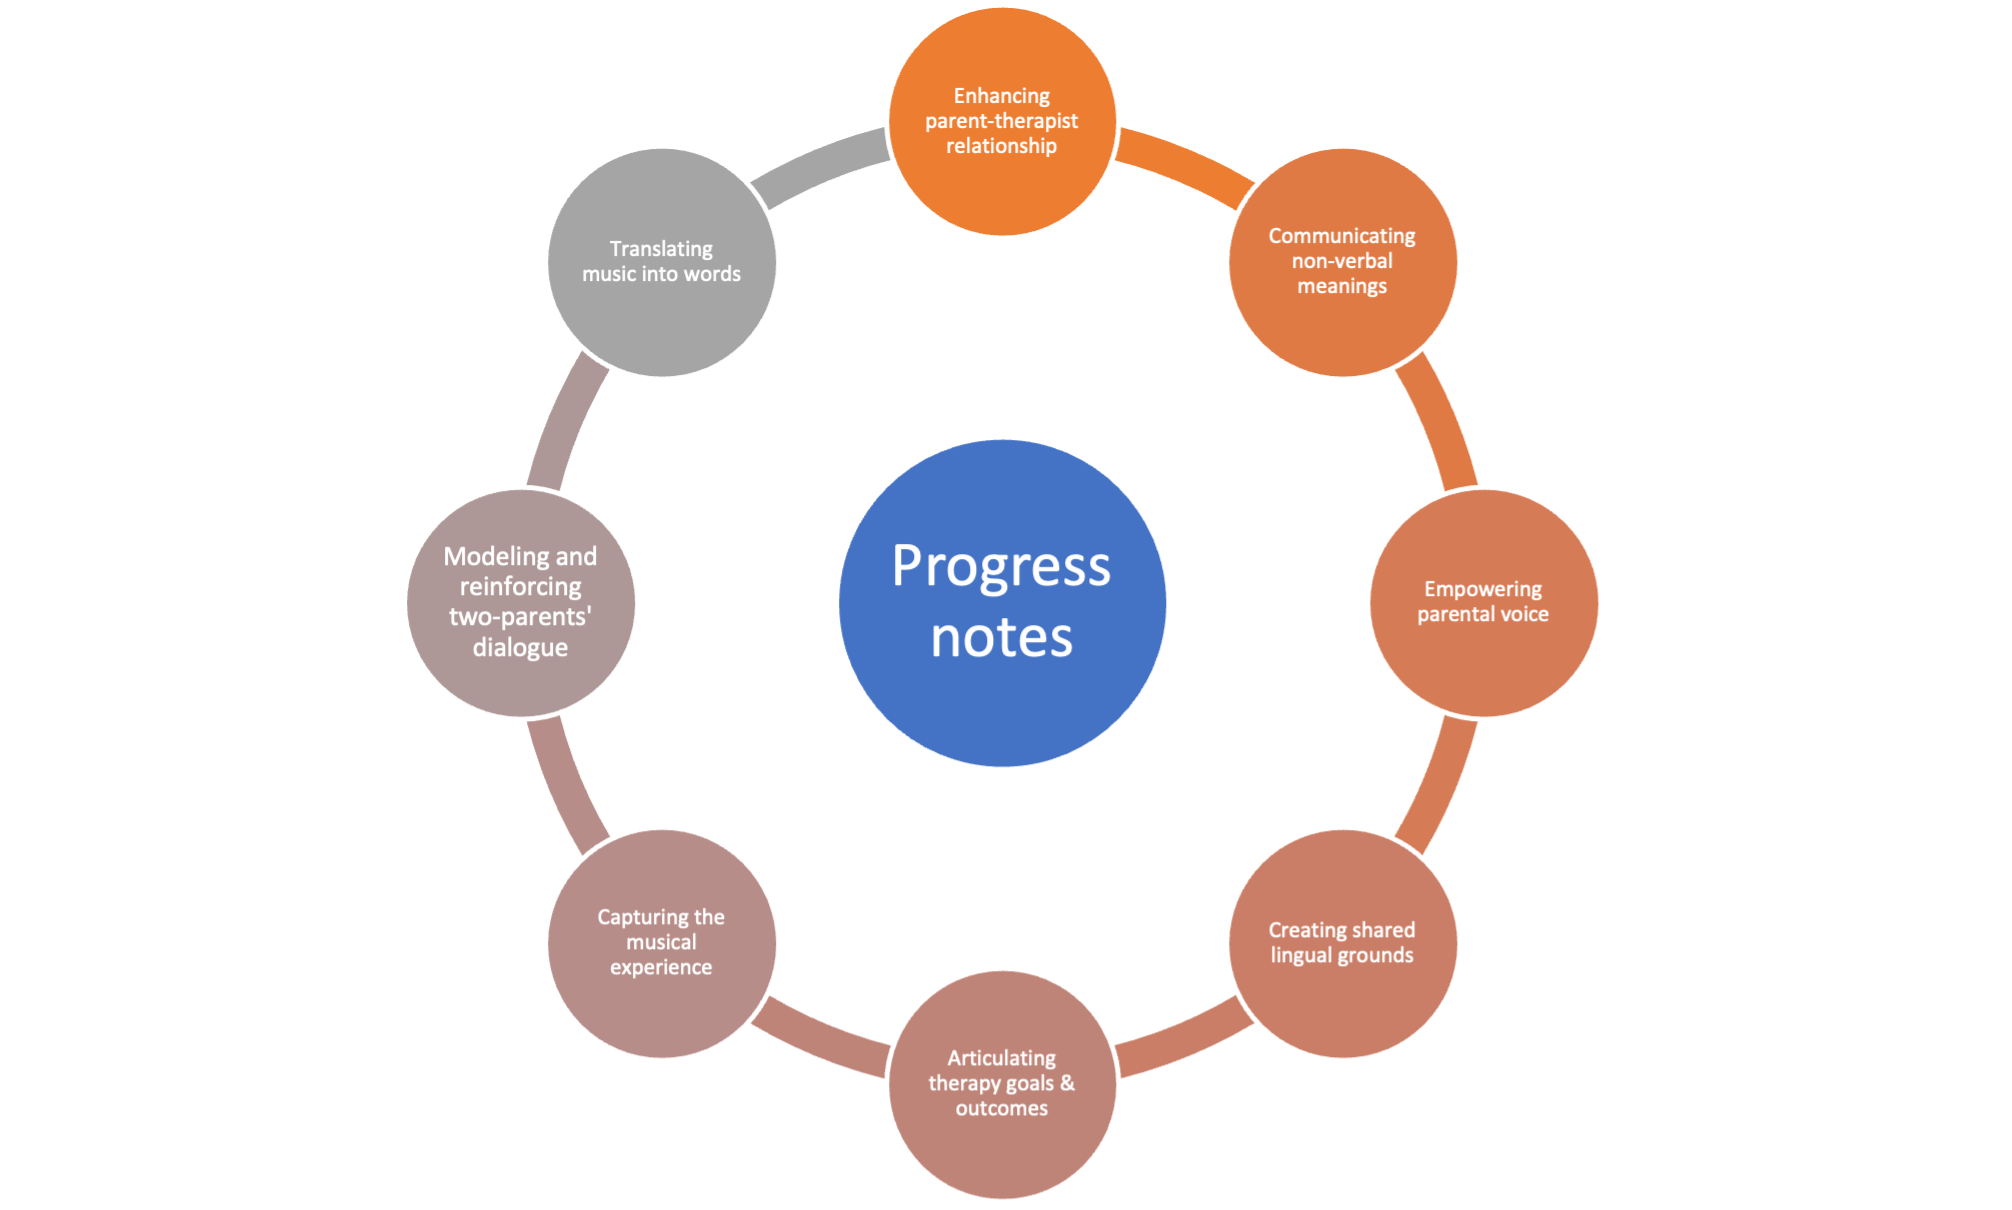
\includegraphics[width=\textwidth]{media/Picture1.png}
    \caption{Layers of Meaning Embedded in Progress Notes}
  \end{fullwidth}
\end{figure*}

The vignette described here captures a multilayered yet unfulfilled moment (see Figure 1) in which the therapist missed an opportunity with the parent to communicate several aspects of the music therapy experience. These aspects related to therapy, to the parent-child relationship as well as therapist-caretaker relationship, and to the musical experience per-se. The progress note, in this case, could have been utilized to convey and contain the non-verbal behaviors as experienced by the therapist. In addition, in acknowledgement of the existing cultural and lingual gaps between therapist and parent, the progress note might have been used to establish common lingual grounds (e.g., Hadar, 2022), and for co-creating a shared language when discussing B. Such an approach could be modeled later within the couple's dyadic system (i.e., between B's parents), when talking about their daughter and pondering on her needs together. In her exploration of working as a music therapist with clients of various cultural backgrounds, and as an immigrant music therapist herself, Hadar (2022) reflected on a clinical moment when a plural-lingual approach facilitated the creation of a shared language between the therapist, the mother and her autistic child - perhaps a moment of shared “\emph{musilanguage”} (Van Puyvelde \& Franco, 2015). Whereas the nuanced attention to the lingual and musical gaps existing between the parent and therapist facilitated the emergence of a shared experience (Hadar, 2022), the lack of attention to such ephemeral qualities led to a very different moment, described in this piece. Inviting the parent to co-create the progress note, (e.g., by reading aloud while writing and inviting them to add their perspectives, rather than handing a completed, enigmatic note), could have served to establish a more equal relation between parent and therapist and to promote the parents' sense of ability and agency while raising a child who is coping with such severe symptoms.

Furthermore, the essence of progress notes relates to issues of reflection and translation: translating to parents' possible meanings in therapy; reflecting with parents on their own thoughts and feelings, as well as sharing the therapist's thoughts and feelings concerning the session; and translating parents' and therapists' visions into operative goals and objectives. In a music therapy setting, this process is further complicated by the need to reflect on the music created in the room and to extract meaning from it. Being a temporal phenomenon, one cannot return to the musical moment once ended (unless it is recorded). This makes the musical moment difficult to capture for the therapist alone and even more challenging to reflect on, in a way that will be sensitive to the parents' musical experience and knowledge. This intricate process of integrating meanings in different languages (i.e., music and verbal language) is a core component of music therapy practice (Lindbald, 2016; Perilli, 2017; Turry, 2009). Shifting between the language of music and verbal languages is at the heart of the music therapy process, regardless of when the progress notes are written, and marks one of the unique possibilities embedded in music therapy. However, the moment when the therapist is consolidating various layers of meaning experienced by themselves and the clients in the session into words and printing them on paper is a beautiful opportunity to exercise and acknowledge this delicate movement in music therapy: the movement between sounds and words, between experience and reflection (Perilli, 2017).



The moment when a musical experience reaches the conscious mind and is being reflected upon is a unique moment when different inner contents might emerge (Lindbald, 2016; Perilli, 2017). Focusing on the meaning of verbal narratives in Guided Imagery Music therapy (GIM), Perilli (2017) emphasized how verbal processing bridges somatic and sensory experiences into conscious knowledge and supports clients in interpreting their musical (and non-musical) experiences in both altered and ordinary states of consciousness, (i.e., both in the here and now moment of experience, as well as a few days later). Perilli's distinction between the moment of experience and the reflective moment is comparable to the difference between reflecting on a musical interaction in the moment versus reflecting on it in the progress note at the end of a session. In this respect, writing a progress note through co-creating, co-reflecting and co-translating different musical moments together with families might sharpen the music therapists' attention to such reflective process in a broader sense. The significance of progress notes in music therapy therefore lies not only in their role as a means of communication and sharing with parents, but also in their capacity to emphasize the delicate and reflective processes inherent to music therapy practice, which involves the art of translating music into words.


\section{Conclusions}



This paper aimed to dissect the potential meanings of progress notes in music therapy settings, and to identify the opportunities missed when such hidden potential is under-evaluated. Ultimately, this piece highlighted the vast potential of progress notes in supporting the delicate movement between sound and words, and between experiential and reflective levels in music therapy practice. It is hoped that this vignette will entice further examination of different gestures and behaviors within the therapeutic encounter, which hold great significance for the therapeutic relationship and for therapy success altogether, but which occasionally remain unnoticed.







\section{References}



\hspace*{\parindent}Chifa, M., Hadar, T., Politimou, N., Reynolds, G., \& Franco, F. (2021). The soundscape of neonatal intensive care: A mixed-methods study of the parents' experience. \emph{Children}, \emph{8}(8), Article 644. \href{https://doi.org/10.3390/children8080644}{https://doi.org/10.3390/children8080644}\underline{.}



Epstein, S., Elefant, C., \& Ghetti, C. (2022). Israeli parents' lived experiences of music therapy with their preterm infants post-hospitalization. \emph{The Journal of Music Therapy, 59}(3), 239--268. \href{https://doi.org/10.1093/jmt/thac006}{https://doi.org/10.1093/jmt/thac006}



Hadar, T. (2022). “What sound does a cat make in Cantonese?”: Advocating for lingual plurality in music therapy settings. \emph{Voices: A World Forum for Music Therapy}, \emph{22}(3). https://doi.org/10.15845/voices.v22i3.3483



Hadar, T., Politimou, N. \& Franco, F. (2023). Singing or playing the flute? Parents' perceptions of two different settings for parent-infant music groups. \emph{Psychology of Music}. \href{https://doi.org/10.1177/03057356231166759}{https://doi.org/10.1177/03057356231166759}



Inhestern, L., Peikert, M. L., Krauth, K. A., Escherich, G., Rutkowski, S., Kandels, D., \& Bergelt, C. (2020). Parents' perception of their children's process of reintegration after childhood cancer treatment. \emph{PloS One, 15}(10), e0239967--e0239967. https://doi.org/10.1371/journal.pone.0239967



Kobus, S., Diezel, M., Huening, B., Dewan, M. V., Felderhoff-Mueser, U., \& Bruns, N. (2021). Parents' perception of family-centered music therapy with stable preterm infants. \emph{International Journal of Environmental Research and Public Health, 18}(23), Article 12813. \href{https://doi.org/10.3390/ijerph182312813}{https://doi.org/10.3390/ijerph182312813}



Lindblad, K. (2016). Verbal dialogue in music therapy: A hermeneutical analysis of three music therapy sessions. \emph{Voices: A World Forum for Music Therapy,}\emph{ }\emph{16}(1). \href{https://doi.org/10.15845/voices.v16i1.842}{https://doi.org/10.15845/voices.v16i1.842}



Perilli, G. G. (2017). \emph{Assessment and Evaluation of Narratives in Guided Imagery and Music (GIM)}. Barcelona Publishers.



Romani, P. W., Ladyga, R., \& McCleary, M. (2023). Use of didactic training and feedback to improve quality and acceptability of progress notes written by direct-care staff on a psychiatric inpatient unit. \emph{Behavioral Interventions, 38}(2), 427-- 436. https://doi.org/10.1002/bin.1927



Salloum, A., Dorsey, C. S., Swaidan, V. R., \& Storch, E. A. (2015). Parents' and children's perception of parent-led Trauma-Focused Cognitive Behavioral Therapy. \emph{Child Abuse \& Neglect}, \emph{40,} 12--23. \href{https://doi.org/10.1016/j.chiabu.2014.11.018}{https://doi.org/10.1016/j.chiabu.2014.11.018}



Turry, A. (2009). Integrating musical and psychological thinking: The relationship between music and words in clinically improvised songs. \emph{Music and Medicine}, \emph{1}(2), 106-116.



Van Puyvelde, M. \& Franco, F. (2015). The interaction of music and language in theontogenesis of human communication: A multimodal parent-infant co-regulation system. In: R. Timmers, N. Dibben, Z. Eitan, R. Granot, T.Metcalfe, A. Schiavio, \& V. Williamson (Eds.). International Conference on the Multimodal Experience of Music. \emph{Proceedings of ICMEM 2015}. Sheffield:HRI Online Publications, 0000. Available online at:<http://hridev1.shef.ac.uk/openbook/chapter/ICMEM\_39>






\end{document}